The derivation of fragility models requires the description of the characteristics of the system to be assessed. A full characterisation of a structure can be done with an analytical structural model, but for the use in some fragility methodologies its fundamental features can be adequately described using a pushover curve, which describes the nonlinear behaviour of each input structure subjected to a horizontal lateral load.

Different methodologies require the pushover curve to be expressed with different parameters and to be combined with additional building information (e.g. period of the structure, height of the structure). The following input models have thus been implemented in the Risk Modeller's Toolkit:\\

\begin{enumerate}
 \item \verb=Base Shear vs Roof Displacement=
 \item \verb=Base Shear vs Floor Displacements=
 \item \verb=Spectral acceleration vs Spectral displacement=\\
\end{enumerate}

Within the description of each fragility methodology provided below, the required input model and the additional building information are specified. Moreover some methodologies give the user the chance to select the input model that fits better to the data at his or her disposal. Considering that different methodologies sharing the same input model may need different parameters, not all the information defined in the input file are necessarily used by each method. The various inputs are currently being stored in a \verb=csv= file (tabular format), as illustrated in the following Sections for each input model.

Once the pushover curves have been defined in the input file and uploaded in the IPython notebook, they can be visualised with the following function:

\begin{Verbatim}[frame=single, commandchars=\\\{\}, samepage=true]
utils.plot_capacity_curves(capacity_curves)
\end{Verbatim}


\subsubsection{Base Shear vs Roof Displacement}
\label{subsubsec:VB-Droof}
Some methodologies require the pushover curve to be expressed in terms of Base Shear vs Roof Displacement (e.g. Dolsek and Fajfar 2004 in Section~\ref{subsec:DolsekFajfar}, SPO2IDA in Section~\ref{subsec:SPO2IDA}). Additional building information is needed to convert the pushover curve (referring to a Multi Degree of Freedom, MDoF, system) to a capacity curve (Single Degree of Freedom, SDoF, system).\\

When the pushover curve is expressed in terms of Base Shear vs Roof Displacement, the user has to set the \verb=Vb-droof= variable to \verb=TRUE= in the input file, and define whether it is an idealised (e.g. bilinear) or a full pushover curve (i.e. with many pairs of base shear and roof displacement values), setting the variable \verb=Idealised= to \verb=TRUE= or \verb=FALSE= respectively. Then the following information about the structures to be assessed is needed:\\

\begin{enumerate}
\item \verb=Periods=, first period of vibration T$_1$.
\item \verb=Ground height=, height of the ground floor.
\item \verb=Regular height=, height of the regular floors.
\item \verb=Gamma participation factors=, modal participation factor $\Gamma_1$ of the first mode of vibration, normalised with respect to the roof displacement.
\item \verb=Number storeys=, number of storeys.
\item \verb=Weight=, weight assigned to each structure for the derivation of fragility models for many buildings.
\item \verb=Vbn=, the base shear vector of the n$^{th}$ structure.
\item \verb=droofn=, the roof displacement vector of the n$^{th}$ structure. \\
\end{enumerate}

Only bilinear and quadrilinear idealisation shapes are currently supported to express the pushover curve in an idealised format, therefore the $V_b$ and $d_{roof}$ vectors should contain 3 or 5 $V_b$-$d_{roof}$ pairs, respectively, as described in the following lists and illustrated in Figures \ref{fig:bilinear} and \ref{fig:quadrilinear}.\\

Bilinear idealisation inputs:
\begin{itemize}
\item Displacement vector: displacement at Vb = 0 ($d_0$), yielding displacement ($d_1$), ultimate displacement ($d_2$).
\item Base Shear vector: Vb = 0, base shear at yielding displacement ($Vb_1$), base shear at ultimate displacement ($Vb_2$ = $Vb_1$).\\
\end{itemize}
\begin{figure}[htb]
  \centering
      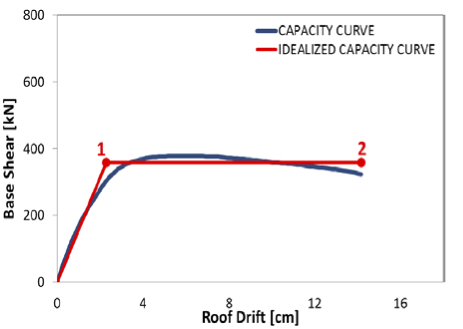
\includegraphics[width=9cm]{figures/bilinear.jpg}
  \caption{Inputs for bilinear idealisation of pushover curve.}
  \label{fig:bilinear}
\end{figure}

Quadrilinear idealisation inputs:
\begin{itemize}
\item Displacement vector: displacement at Vb = 0 ($d_0$), yielding displacement ($d_1$), displacement at maximum base shear ($d_2$), displacement at onset of residual force plateau ($d_3$), ultimate displacement ($d_4$).
\item Base Shear vector: Vb = 0, base shear at yielding displacement ($Vb_1$), maximum base shear ($Vb_2$), residual force ($Vb_3$) and force at ultimate displacement ($Vb_4$).\\
\end{itemize} 

\begin{figure}[htb]
  \centering
      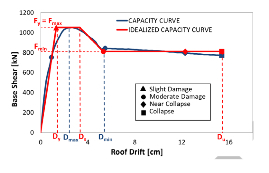
\includegraphics[width=9cm]{figures/quadrilinear.jpg}
  \caption{Inputs for quadrilinear idealisation of pushover curve.}
  \label{fig:quadrilinear}
\end{figure}

An example of an input \verb=csv= file for the derivation of a fragility model for a set of two structures, whose pushover curves are expressed with an idealised bilinear shape, is presented in Table \ref{table:Vb-droof_input}.

\begin {table}[htb]
\caption{Example of a Base Shear-Roof Displacement input model.}
\label{table:Vb-droof_input}
\begin{center}
  \begin{tabular}{ | c | c | c | c | c |}
  \hline
    Vb-droof & TRUE &  &  \\ \hline
    Vb-dfloor & FALSE & & \\ \hline
    Sd-Sa & FALSE & & \\ \hline
    Idealised & TRUE & & \\ \hline
    Periods [s] & 1.61 & 1.5 & \\ \hline
    Ground heights [m] & 7 & 6.5 & \\ \hline
    Regular heights [m] & 2.7 & 3.0 & \\ \hline
    Gamma participation factors & 1.29 & 1.4 & \\ \hline
    Number storeys & 6 & 6 & \\ \hline
    Weights & 0.5 & 0.5 & \\ \hline
    Vb1 [kN] & 0 & 2090 & 2090 \\ \hline
    droof1 [m] & 0 & 0.1 & 0.6 \\ \hline
    Vb2 [kN] & 0 & 1700 & 1700 \\ \hline
    droof2 [m] & 0 & 0.08 & 0.5 \\ \hline
  \end{tabular}
\end{center}
\end{table}

\subsubsection{Base Shear vs Floor Displacements}
\label{subsubsec:VB-Dfloor}
A modification of the previous input model is the Base Shear vs Floor Displacements input type. In this case the conversion to a SDoF capacity curve is still based on the roof displacement, but a mapping scheme between the roof displacement and inter-storey drift at each floor level is also derived, so that the overall deformation state of the structure corresponding to a given roof displacement can be checked.\\
When the pushover curve is expressed in terms of Base Shear vs Floor Displacements, the user has to set the \verb=Vb-floor= variable to \verb=TRUE= in the input file. Only full pushover curves can be input, therefore the variable \verb=Idealised= should be set to \verb=FALSE=. Then the following information about the structures to be assessed is needed:\\

\begin{enumerate}
\item \verb=Periods=, first period of vibration T$_1$.
\item \verb=Ground height=, height of the ground floor.
\item \verb=Regular height=, height of the regular floors.
\item \verb=Gamma participation factors=, modal participation factor $\Gamma_1$ of the first mode of vibration, normalised with respect to the roof displacement.
\item \verb=Number storeys=, number of storeys.
\item \verb=Weight=, weight assigned to each structure for the derivation of fragility models for many buildings.
\item \verb=Vbn=, the base shear vector of the n$^{th}$ structure.
\item \verb=dfloorn-1=, the displacement vector of the 1$^{st}$ floor of the n$^{th}$ structure.
\item \verb=dfloorn-2=, the displacement vector of the 2$^{nd}$ floor of the n$^{th}$ structure.
\item \verb=dfloorn-k=, the displacement vector of the k$^{th}$ floor of the n$^{th}$ structure. \\
\end{enumerate}

An example of an input \verb=csv= file for the derivation of a fragility model for a set of two structures, is presented in Table~\ref{table:Vb-dfloor_input}.

\begin {table}[htb]
\caption{Example of a Base Shear-Floor Displacements input model.}
\label{table:Vb-dfloor_input}
\begin{center}
  \begin{tabular}{ | c | c | c | c | c | c | c | c |}
  \hline
    Vb-droof & TRUE &  &  & & & \\ \hline
    Vb-dfloor & FALSE & & & & &  \\ \hline
    Sd-Sa & FALSE & & & & & \\ \hline
    Idealised & FALSE & & & & & \\ \hline
    Periods [s] & 1.61 & 1.5 & & & & \\ \hline
    Ground heights [m] & 7 & 6.5 & & & & \\ \hline
    Regular heights [m] & 2.7 & 3.0 & & & & \\ \hline
    Gamma participation factors & 1.29 & 1.4 & & & & \\ \hline
    Number storeys & 6 & 6 & & & & \\ \hline
    Weights & 0.5 & 0.5 & & & & \\ \hline
    Vb1 [kN] & 0	& ...	& 50	& 94	& 118	& \\ \hline
	  dfloor1-1 [m] & 0.002	& ...	& 0.05	& 0.09	& 0.11	& \\ \hline
	  dfloor1-2 [m] & 0.004	& ...	& 0.12	& 0.16	& 0.20	& \\ \hline
    Vb2 [kN] & 0	& ...	& 79	& 100	& 105	& 150 \\ \hline
    dfloor2-1 [m] & 0.006 &	...	& 0.018	& 0.023	& 0.05	& 0.1 \\ \hline
	dfloor2-2 [m] & 0.008	& ... &	0.023	& 0.030	& 0.038	& 0.15 \\ \hline
  \end{tabular}
\end{center}
\end{table}

\subsubsection{Spectral acceleration vs Spectral displacement}
\label{subsubsec:Sa-Sd}
Some methodologies work directly with capacity-curves (Spectral acceleration vs Spectral displacement) of SDoF systems (e.g. N2 in Section~\ref{subsec:N2}, CSM in Section~\ref{subsec:CSM}), so that the user can provide his or her own conversion of pushover curves, or can use the "Conversion from MDOF to SDOF" module in Section~\ref{sec:mdof_to_sdof}.\\
When the pushover curve is expressed in terms of Spectral acceleration vs Spectral displacement, the user has to set the \verb=Sd-Sa= variable to \verb=TRUE= in the input file. Then the following information about the structures to be assessed is needed:\\

\begin{enumerate}
\item \verb=Periods=, first periods of vibration T$_1$.
\item \verb=Heights=, heights of the structure.
\item \verb=Gamma participation factors=, modal participation factors $\Gamma_1$ of the first mode of vibration.
\item \verb=Sdy=, the yielding spectral displacements.
\item \verb=Say=, the yielding spectral accelerations.
\item \verb=Sdn [m]=, the Sd vector of the n$^{th}$ structure.
\item \verb=San [g]=, the Sa vector of the n$^{th}$ structure. \\
\end{enumerate}

An example of an input \verb=csv= file for the derivation of a fragility model for a set of three structures, is presented in Table \ref{table:Sa-Sd_input}.

\begin {table}[htb]
\caption{Example of a Spectral acceleration-Spectral displacement input model.}
\label{table:Sa-Sd_input}
\begin{center}
  \begin{tabular}{ | c | c | c | c | c |}
  \hline
	Vb-droof &	FALSE & &  \\ \hline
	Vb-dfloor & 	FALSE & & \\ \hline
	Sd-Sa &	TRUE & & \\ \hline
	Periods [s] &	1.52 &	1.63 &	1.25 \\ \hline
	Heights [m]	& 6 &	6	& 6 \\ \hline
	Gamma participation factors	& 1.24 &	1.24 &	1.24 \\ \hline
	Sdy [m] & 	0.0821 & 	0.0972 &	0.0533\\ \hline
	Say [g]	& 0.143	& 0.14723	& 0.13728 \\ \hline
	Sd1 [m]	& 0 &	0.0821	& 0.238 \\ \hline
	Sa1 [g]	& 0	& 0.143	& 0.143 \\ \hline
	Sd2 [m] &	0 & 0.0972	& 0.264 \\ \hline
	Sa2 [g]	& 0	& 0.14723	& 0.14723 \\ \hline
	Sd3 [m]	& 0	& 0.0533	& 0.0964 \\ \hline
	Sa3 [g]	& 0	& 0.13728	& 0.13728 \\ \hline
  \end{tabular}
\end{center}
\end{table}